%------------------------------- CHAPTER NAME --------------------------------
\chapter{Take-off performance}
Although the take-off field length may seem like a performance characteristic of secondary importance, it is very often one of the critical design constraints. If the required runway length is too long, the aircraft cannot take-off with full fuel or full payload and its economics are compromised.
%
So take-off performance play a significant role in the preliminary design of an aircraft because they are both design requirements, specified by the FAR and by the customer, to be fulfilled, both driving parameters in the definition of the design point. 
%
%-------------------------- THEORETICAL BACKGROUND ---------------------------
\section{Theoretical background}
%
\begin{figure}[!b]
\centering
\includegraphics[keepaspectratio, width=1.02\textwidth]{TakeOffRun}
\caption{Scheme of an aircraft take-off run}
\label{fig:TOrun}
\end{figure}
%
The take-off may be considered as made up of two parts: a ground run and an air run, as shown schematically in figure~\ref{fig:TOrun}. The simplest description of the take-off process is that the engine thrust is increased to the take-off level at x = 0 and the brakes are released to begin acceleration down the runway. At some point, the pilot commands rotation of the aircraft which lifts the nose wheel from the ground and allows to achieve the take-off angle of attack; in this way the aircraft lift can grows faster and, when it is equal to the aircraft maximum take-off weight, the aircraft can lifts completely from the ground and begins climbing. The point at which it reaches an altitude of 35 \si{ft} (10.7 \si{\meter}), is considered, for an aircraft which refers to the FAR-25, the end of the take-off run. 
%
This is the usual situation for take-off; subsequently, the modifications to safely deal with a take-off emergency, such as an engine failure, will be discussed.
%
%-----------------------------AOE Take-Off subsection-----------------------------
\subsection{\gls{acr:AOE} take-off run}
In order to deal with the calculation of the take-off run distance, a smart strategy is to find out all the foundamentals variables, which describes completely the aircraft state in this phase, and so, to study the dynamic system in exam in a state-space representation.
%
\noindent
To find out these state variables it is necessary to analyze aircraft equations of motion during take-off phases, these latter described as follows.
\begin{itemize}
\item \textbf{Ground roll phase}: starting from standstill with brakes released and at maximum power output, the aircraft accelerates on the runway, with constant angle of attack, until it reaches a speed equals to the rotation speed V\textsubscript{Rot}; after that the following subphase begin.
%
\begin{itemize}
\item \textbf{Rotation phase}: a short phase in which the pilot gives an assigned pitching law to lift the aircraft nose and, as a result, increasing the angle of attack. This phase ends when the load factor is equal to 1, meaning that the lift has reached the value of the maximum take-off weight, and the relative lift-off speed is indicated with V\textsubscript{LO}. 
%
\end{itemize}
%
\item \textbf{Airborne phase}: is the phases in which the aircraft, once it has lifted from the ground, gains altitude until it reaches the obstacle height of 35 \si{ft} (10.7 \si{\meter}) imposed by the FAR-25. This phase begin at V\textsubscript{LO} and ends at the speed related to the obstacle overcoming, indicated with V\textsubscript{2}; furthermore it can be divided into the followngs two subphases:
%
\begin{itemize}
\item \textbf{Transition phase}: in which the aircraft rotates in order to increase the climb angle ($\gamma$) with the result of increasing the angle of attack and the relative lift coefficient, which should not surpass a safety value of the 90\% of the maximumlift coefficient in take-off configuration. This sub-phase ends when the desidered climb speed is reached.
%
\item \textbf{Climb-out to the obstacle phase}: in which the aircraft climbs at constant climb angle until the obstacle is surpassed.
\end{itemize}
\end{itemize}
%
\noindent
For more information regarding take-off equations of motion during each of the previously described phases, the reader can refer to~\cite{McCormick}.

\bigskip
\noindent
The set of \gls{acr:ODE} that models the take-off run is written in the following form:

\begin{equation}\label{eq:Take:Off:System:Dynamics:A}
    \LEFTRIGHT\lcbrace\rcbrace{\begin{array}{c}\dot{s}\\[2pt] \dot{V} \\[2pt] \dot{\gamma} \\[2pt] \dot{h} \end{array}}
= 
    \LEFTRIGHT\lcbrace\rcbrace{\begin{array}{l}
       f_1 \big(\, s,\, V,\, \gamma,\, h \,; \, \alpha \big) \\[4pt]
       f_2 \big(\, s,\, V,\, \gamma,\, h \,; \, \alpha \big) \\[4pt]
       f_3 \big(\, s,\, V,\, \gamma,\, h \,; \, \alpha \big) \\[4pt]
       f_4 \big(\, s,\, V,\, \gamma,\, h \,; \, \alpha \big)
    \end{array}}
\qquad
    \text{with}\quad
    \LEFTRIGHT\lcbrace.{\begin{array}{l} x_1 = s\\[2pt] x_2 = V \\[2pt] x_3 = \gamma \\[2pt] x_4 = h \end{array}}
\qquad
    \text{and}\quad
    u = \alpha
\end{equation}
%
\noindent
These equations can be also written in a more concise way as shown below.
%
\begin{equation}
\label{eq:Take:Off:System:Dynamics:B}
\dot{\vec{x}} = \vec{f}\big(\, \vec{x}\,;\,u \,\big)
\end{equation}
%
\noindent
The unknown $\vec{x} = [\mspace{2mu} x_1,\, x_2,\, x_3,\, x_4 \mspace{2mu}]^{\text{T}}$ is the vector of state variables. The input $u(t)$ is a given function of time, for $0 \leq t \leq t_{\text{final}}$, that corresponds to an assumed time history of the angle of attack during take-off.
%
The right-hand sides of system (\ref{eq:Take:Off:System:Dynamics:A}) are defined by the following functions:
%
\begin{subequations}\label{eq:Take:Off:System:Dynamics:RHS:functions}
\begin{equation}\label{eq:Take:Off:System:Dynamics:RHS:functions:A}
f_1 \big(\, \vec{x}\,,\,u \,\big) =  x_2
\end{equation}
%
\begin{equation}\label{eq:Take:Off:System:Dynamics:RHS:functions:B}
f_2 \big(\, \vec{x}\,,\,u \,\big) =
  \frac{g}{W}
    \LEFTRIGHT\lcbrace.{
      \begin{array}{l@{\rule{2em}{0pt}}l} 
        T(x_2) - D(x_2,u) - \mu \big[ W - L(x_2,u) \big]
          & \text{if} \;\, \mathcal{S}(x_2 , u) < 1
        \\[1em]
        T(x_2) \cos u - D(x_2,u) - W \sin x_3
          & \text{if} \;\, \mathcal{S}(x_2 , u) \geq 1
      \end{array}
    }  
\end{equation}
%
\begin{equation}\label{eq:Take:Off:System:Dynamics:RHS:functions:C}
f_3 \big(\, \vec{x}\,,\,u \,\big) =
  \frac{g}{W\,x_2}
    \LEFTRIGHT\lcbrace.{
      \begin{array}{l@{\rule{2em}{0pt}}l} 
        0
          & \text{if} \;\, \mathcal{S}(x_2 , u) < 1
        \\[1em]
        L(x_2,u) + T(x_2)\sin u - W \cos x_3
          & \text{if} \;\, \mathcal{S}(x_2 , u) \geq 1
      \end{array}
    }  
\end{equation}
%
\begin{equation}\label{eq:Take:Off:System:Dynamics:RHS:functions:D}
f_4 \big(\, \vec{x}\,,\,u \,\big) =  x_2 \, \sin x_3
\end{equation}
%
\noindent
The thrust $T(x_2)$ is calculated by means of the interpolating function $T_{\text{tab}}\big(V_{\text{a}}\big)$ based on a table lookup algorithm, where $V_{\text{a}} = V + V_{\text{w}}$ is the airspeed and $V_{\text{w}}$ is the wind speed (horizontal component, positive if opposite to the aircraft motion).
%
The drag $D$ and lift $L$, as functions of airspeed $V_{\text{a}}$ and angle of attack, are given by the following conventional formulas.
%
\begin{equation}\label{eq:Take:Off:System:Dynamics:RHS:functions:E}
D(x_2,u) = \frac{1}{2} \, \rho \, \big( x_2 + V_{\text{w}}\cos x_3 \big)^2 \,S \, C_D\big( u \big)
\end{equation}
%
\begin{equation}\label{eq:Take:Off:System:Dynamics:RHS:functions:E}
L(x_2,u) = \frac{1}{2} \, \rho \, \big( x_2 + V_{\text{w}}\cos x_3 \big)^2 \,S \, C_L\big( u \big)
\end{equation}
%
\noindent
The switching function $\mathcal{S}$ of aircraft velocity and angle of attack is defined as follows:
%
\begin{equation}\label{eq:Take:Off:System:Dynamics:RHS:functions:D}
\mathcal{S}(x_2 , u) = \frac{L(x_2,u)}{W \cos x_3}
\end{equation}
\end{subequations}
%
\noindent
The formulas (\ref{eq:Take:Off:System:Dynamics:RHS:functions}) make the system (\ref{eq:Take:Off:System:Dynamics:B})  a closed set of ODEs.
%
\noindent
When the function $u(t)$ is assigned and the system is associated to a set of initial conditions, in this particular case equal to $\vec{x}_0 = [\mspace{2mu} 0,\, 0,\, 0,\, 0 \mspace{2mu}]^{\text{T}}$, a well-posed \gls{acr:IVP} is formed, which can be solved numerically.
%
In table~\ref{tab:Take:Off:Speeds:FAR25} are reported the take-off characteristic speeds and their corresponding requirements as defined by FAR~25.
%
\begingroup
\begin{longtable}[H]{lll}
\label{tab:Take:Off:Speeds:FAR25}\\
\toprule
Speed & Description & Requirement
\\ \midrule
\endfirsthead
%
\multicolumn{3}{l}%
  {\relsize{-1}({\itshape continued from previous page})}\\
\toprule
Speed & Description & Requirement
\\ \midrule
\endhead
%
\midrule \multicolumn{3}{r}{{\relsize{-1}\itshape continued on next page}}
\endfoot
%
\bottomrule
\caption[Take-off speeds and FAR~25 requirements]{Take-off speeds and FAR~25 requirements}
\endlastfoot
%
$V_\mathrm{S}$ & aircraft stalling speed in take-off configuration & ---
\\
$V_\mathrm{MC}$ & minimum control speed with one engine inoperative (OEI) & ---
\\
$V_1$ & OEI decision speed & $\geq V_\mathrm{mc}$
\\
$V_\mathrm{Rot}$ & rotation speed & $>1.05\, V_\mathrm{MC}$
\\
$V_\mathrm{MU}$ & minimum unstick speed for safe flight & $\geq V_\mathrm{S}$
\\
$V_\mathrm{LO}$ & lift-off speed & $> 1.10 \, V_\mathrm{MU}$
\\
                &                & $> 1.05 \, V_\mathrm{MU}$ (OEI)
\\
$V_2$ & take-off climb speed at \SI[round-precision=0]{35}{ft} & $> 1.20 \, V_\mathrm{S}$
\\
                &                & $> 1.10 \, V_\mathrm{MC}$
\end{longtable}
\endgroup
%
\noindent
It has to be highlithed that the drag coefficient $C_D$ that appears in (\ref{eq:Take:Off:System:Dynamics:RHS:functions:E}) can be modelled as:
%
\begin{equation}\label{eq:CD:A}
C_D = C_{D0} + \left(\upDelta C_{D0}\right)_{\text{flap}+\text{lg}} +  K_g\ \frac{C_L^2}{\pi \AR e}
\end{equation}
%
with $\left(\upDelta C_{D0}\right)_{\text{flap}+\text{lg}}$ due to flap, as shown in subparagraph~\ref{subpar:DCD0}, and landing gears, which contribution is usually about $0.010 \div 0.015$; moreover $C_L$ is the one from the lift curve with flaps, and eventually slats, deflected. The term $K_g$ in (\ref{eq:CD:A}) incorporates the ground effect and it is calculated from~\cite{McCormick} using the (\ref{eqn:FifthOrderPoly}) which is a fifth order interpolating function of the  graph in fugure~\ref{fig:McCormickGroundEffect}, where the ratio $h_{\text{W}}/b$ is obtained dividing the height of wing above the ground by the wing span, usually between 0.1 and 0.2 when the aircraft is on the ground and assumed as $h_{\text{W}} \approx h$ durign the airborne.
%
\begin{figure}[H]
\centering
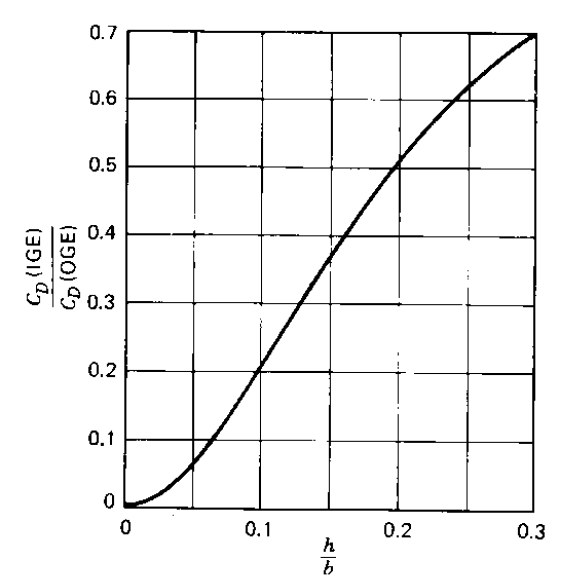
\includegraphics[keepaspectratio, width=0.5\textwidth]{McCormickGroundEffect}
\caption{Gorund effect parameter $K_g$ as function of the $h_{\text{W}}/b$ ratio}
\label{fig:McCormickGroundEffect}
\end{figure}
%
\begin{equation}
K_g=-622.44x^5+624.46x^4-255.24x^3+47.105x^2-0.6378x+0.0055
\label{eqn:FifthOrderPoly}
\end{equation}
%
This polynomial equation has a coefficient of determination $R^2$ of 0.9999 which justifies the approximation.
%
\begin{figure}[!t]
\centering
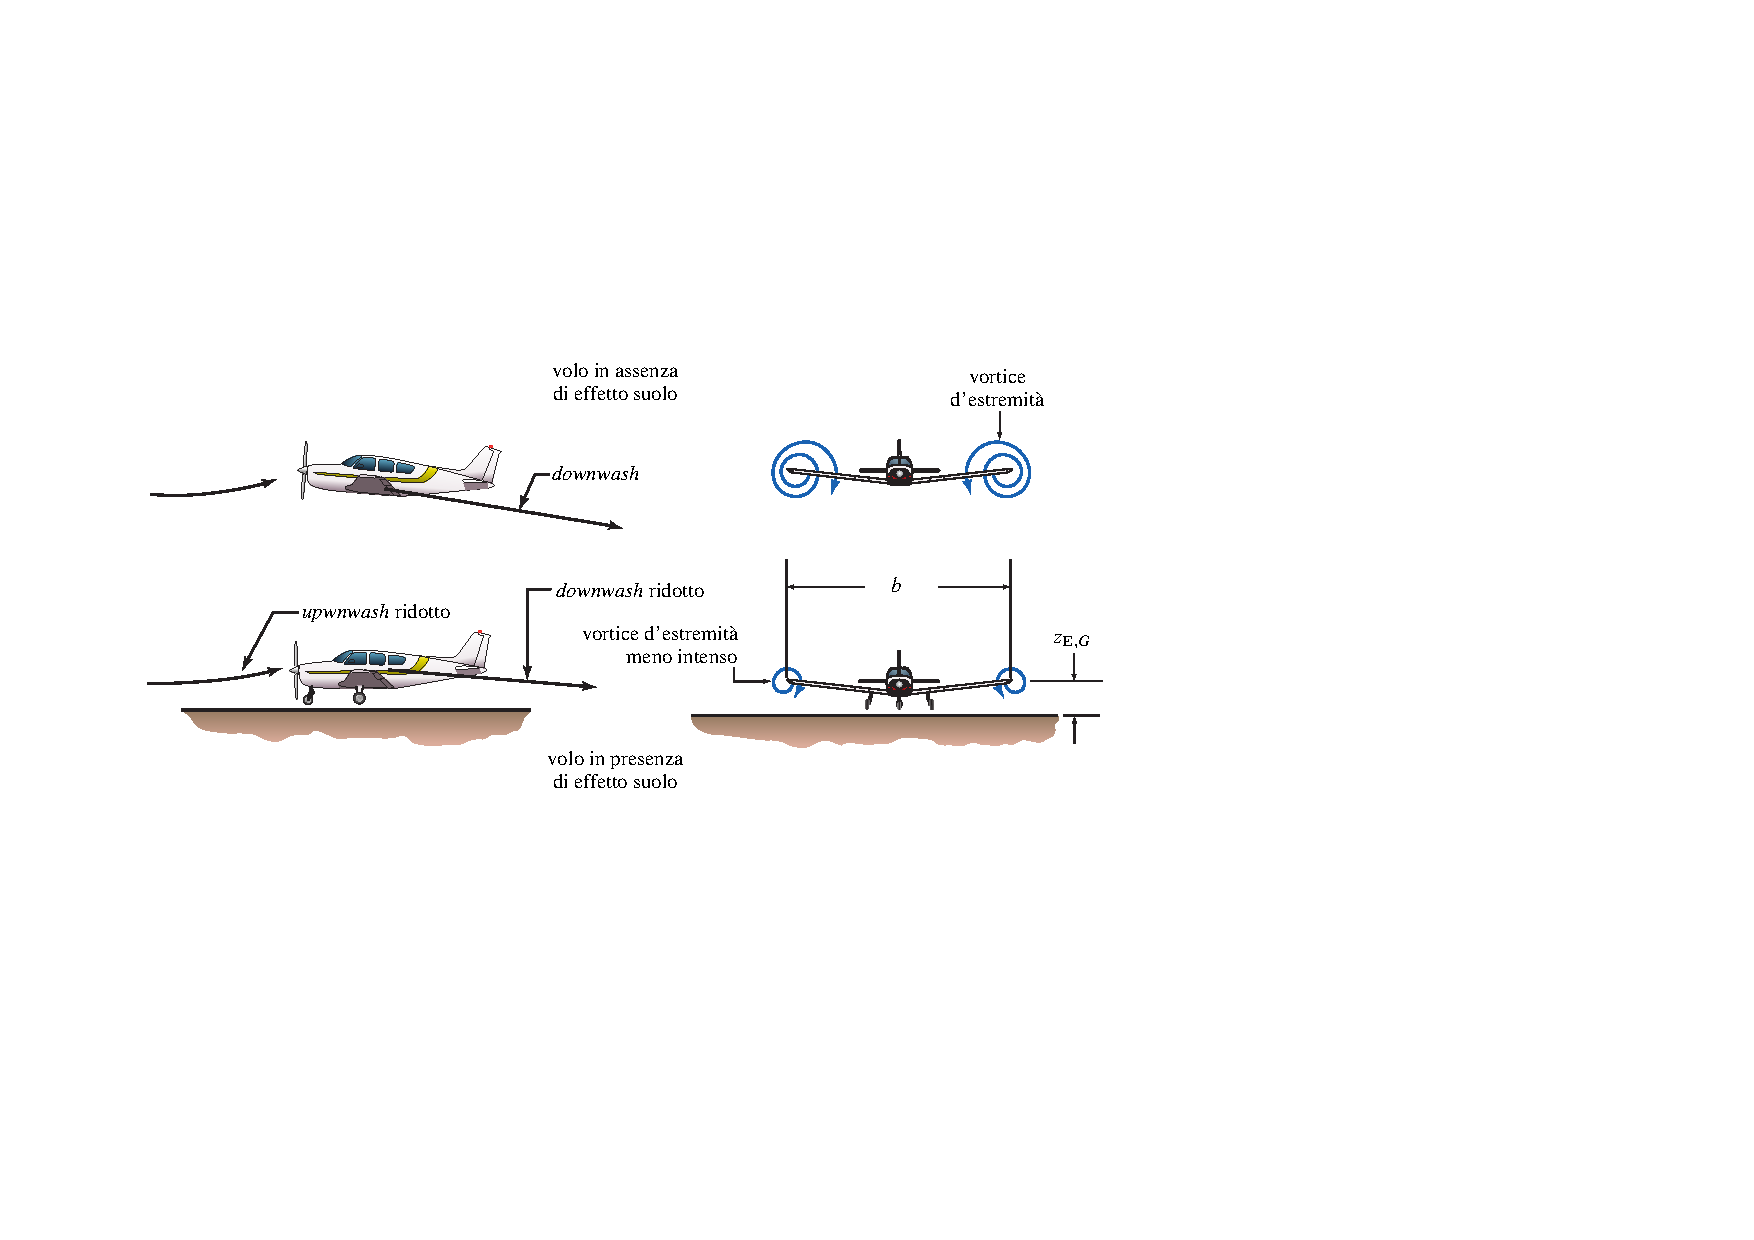
\includegraphics[keepaspectratio, width=\textwidth]{GroundEffect}
\caption{Comparison between flight with and without ground effect}
\label{fig:GroundEffect}
\end{figure}

\bigskip
\noindent
In order to better understand the nature of the ground effect it is convenient to refer to~\cite{nicolai2010fundamentals}, where the ground effect is explained as follows.
%
As the aircraft flies close to the ground, the ground interferes with the horseshoe vortex system trailing behind the wing. Ground effect is often analyzed by putting an image horseshoe vortex system of equal but opposite strength at the same distance $h_{\text{W}}$ below the ground.
%
This image vortex system induces velocities at the wing aerodynamic center, which decreases the strength of the downwash at that point, thereby decreasing the induced angle of attack, $\alpha_i$. Thus, the wing $C_L$ is increased (or more correctly, the lift curve slope increases, giving an increase in $C_L$ for the same geometric angle of attack, $\alpha$) and the induced drag is decreased.
%
This influence of the ground effect is a function of how close the aircraft is to the ground and of the size of the wing.

\bigskip
\noindent
Speaking of the $C_D$, it has also to be noted that, at high $C_L$, the parabolic drag polar it's no longer accurate in describing the drag characteristics of the aircraft so that two correction factors have to be added to the (\ref{eq:CD:A}). These latter triggers only when the $C_L$ is higher than 1.2, as can be seen from the following equation, in which $K_1$ and $K_2$ values depend on the aircraft in exam.
%
\begin{equation}
C_D = C_{D0} + \left(\upDelta C_{D0}\right)_{\text{flap}+\text{lg}} +  K_g\ \frac{C_L^2}{\pi \AR e} + K_1\ \left(C_L-1.2\right) + K_2\ \left(C_L-1.2\right)^2
\end{equation}

\bigskip
\noindent
Focusing, now, on the input law of the angle of attack, the function $u$ can be constructed by picking the time $t_{\text{Rot}}$ when the rotation speed $V_{\text{Rot}}$ is reached along the ground roll; thus the $u (t)$ function can be defined as follows.

\bigskip
\begin{equation}\label{eq:Take:Off:System:Dynamics:Alpha:Law}
u (t) =
    \LEFTRIGHT\lcbrace.{
      \begin{array}{l@{\rule{2em}{0pt}}l} 
        \alpha_{\text{g}}
          & \text{if} \;\, t < t_{\text{Rot}}
        \\[1em]
        \alpha_1(t)
          & \text{if} \;\, t \geq t_{\text{Rot}}
      \end{array}
    }
\end{equation}
%
with a constant $\alpha_{\text{g}}$ during the ground run up to the rotation speed, and a given non-zero law $\alpha_1(t)$ for the post-rotation angle of attack time history. 
%
\begin{figure}[!t]
\centering
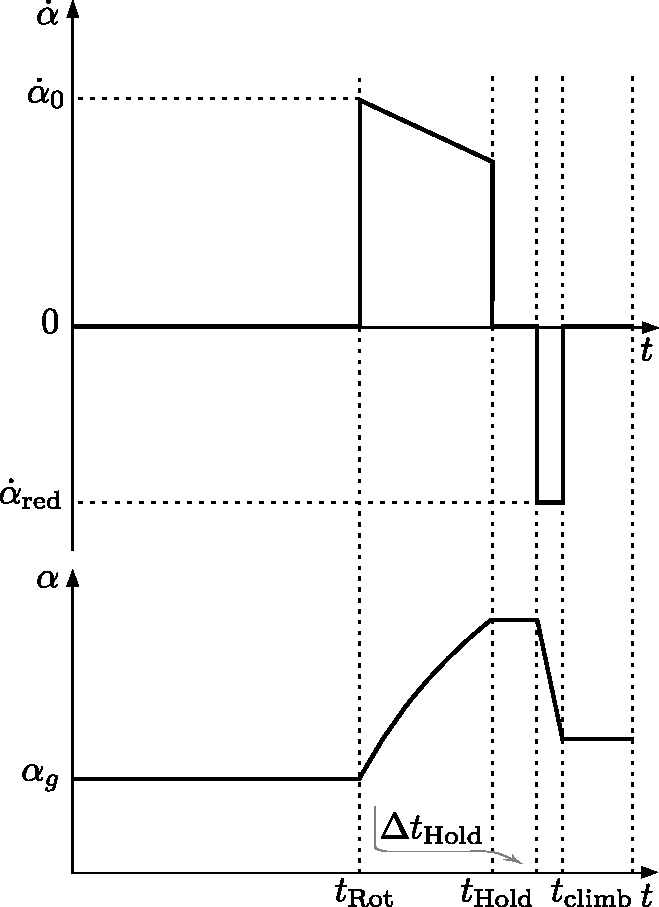
\includegraphics[keepaspectratio, width=0.45\textwidth]{AlphaInputTakeOff}
\caption{Qualitative representation of the angle of attack input law}
\label{fig:AlphaInput}
\end{figure}
%
Figure~\ref{fig:AlphaInput} shows a qualitative representation of the $\alpha_1(t)$ law. As can be seen, after $t_{\text{Rot}}$ the pilot applies an initial angular velocity $\dot\alpha_{0}$, which decreases with time, according to the law written in (\ref{eqn:AlphaDot}) as function of $\alpha$, until the time $t_{\text{Hold}}$ has been reached; this particular instant is related to the achievement of the maximum admitted lift coefficient in take-off, which is set at 90\% of the $C_{L\text{max,TO}}$.
%
\begin{equation}
\dot\alpha=\dot\alpha_0\ \left(1-k_\alpha\ \alpha\right)
\label{eqn:AlphaDot}
\end{equation}
%
\noindent
In equation (\ref{eqn:AlphaDot}), the $k_\alpha$ slope is assigned (a good value could be 0.07 ($\si{1/\degree}$)), while the initial angular velocity $\dot\alpha_0$ is calculated as follows.
%
\begin{equation}
\dot\alpha_0=\dfrac{\upDelta\alpha}{\upDelta t_{\text{Rot}}}=\dfrac{\alpha_{\text{LO}}-\alpha_g}{\upDelta t_{\text{Rot}}}
\label{eqn:AlphaDotInitial}
\end{equation}
%
where $\alpha_{\text{LO}}$ can be obtained from the lift curve of the wing, with flaps deflected in take-off configuration, by assigning the $C_{\text{L}_{\text{LO}}}$; this can be derived from the $C_{L\text{max,TO}}$ dividing it by the parameter $K^2_{\text{LO}}$, which represents the quantity that has to be multiplied by $V_{\text{S}}$ in order to obtain $V_{\text{LO}}$ (for example 1.1 with reference to table~\ref{tab:Take:Off:Speeds:FAR25}).

\bigskip
\noindent
From this point on the pilot stops the pitching manouver and keeps the angle of attack constant for an assigned $\upDelta t_{\text{Hold}}$. During this time interval, the lift coefficient is high and, as a result, also the induced drag is high so that aircraft acceleration will reduce. 
%
After this short time interval the pilot has to reduce the angle of attack in order to avoid the acceleration to decrease too much and so an assigned negative angular velocity $\dot\alpha_{\text{red}}$ is applied; the latter assumed to be constant for simplicity. 
%
Finally, since the decrease of $\alpha$ determines also a reduction in $C_L$, the time $t_{\text{climb}}$ will be reached when the load factor is reduced to 1; this means that a balance of the forces, perpendicular to the flight path, has been achieved and so the climb phase, at constant $\gamma$, can begin, leaving $\alpha$ constant and equal to last value reached. 
%
%-----------------------------OEI Take-Off subsection-----------------------------
\subsection{\gls{acr:OEI} take-off run and balanced field lenght}
A good description of the take-off with one engine failure is proposed in \cite{sforza2014commercial}. Here it is explained that in the event of an engine failure during the take-off roll the pilot must decide whether to continue the take-off or, instead, abort the take-off and decelerate to a stop on the runway. Obviously, if the engine failure occurs when the aircraft is traveling very slowly, the aircraft should be kept on the ground and brought to a stop at some safe location off the runway. Conversely, if the engine failure occurs when the aircraft is close to the take-off speed the take-off should be continued. The designer must provide a means for deciding whether it is safer to abort the take-off or continue it.
%
The critical velocity, denoted as $V_{\text{act}}$, is the velocity at which action is taken, not that at which the decision to act is taken. The time between the recognition of an engine failure, which occurs at $V_{\text{ef}}$, and the critical velocity $V_{\text{act}}$, when action is taken is required to be more than one second. Generally this time period, which is set by the reaction time of the pilot, is taken to be about \SI{3}{\second}. If the pilot’s decision is to continue the take-off with one engine inoperative, the distance to the lift-off speed $V_{\text{LO}}$ and to the subsequent climb-out to 35 $\si{ft}$ height above the runway, will obviously be longer than with all engines operating.

\bigskip
\noindent
The calculation of the take-off distance in this situation is quite the same as the one explained previously, with the difference that now there is a discontinuity in thrust due to the broken engine. In particular, the thrust, $T(x_2)$, will still be read from the database but considering a number of engines reduced by one from the time $t_{\text{ef}}$ at which the engine failure occurs.

\bigskip
\noindent
On the other hand, in the case of the aborted take-off the pilot will apply the necessary braking procedures in order to get the maximum permissible deceleration while maintaining adequate control of the airplane’s motion. The portion of the aborted take-off run up to the engine failure velocity $V_{\text{ef}}$ is calculated in the same way as that for the continued take-off, so that the distance is the same in both cases. 
%
From this point on, until the pilot reacts by activating brakes, there is only a discontinuity in thrust due to the failed engine; while, after the time interval in which the pilot decides to abort the take-off, the thrust is set to minimum (ideally zero) and the brakes action provides an higher friction coefficient. During this last phase, the equation (\ref{eq:Take:Off:System:Dynamics:RHS:functions:B}) changes in the following.
%
\begin{equation}\label{eq:Take:Off:System:Dynamics:RHS:functions:Aborted}
f_2 \big(\, \vec{x}\,,\,u \,\big) =\frac{g}{W}\ \big\{ - D(x_2,u) - \mu_{\text{brakes}} \big[ W - L(x_2,u) \big]\big\} 
\end{equation}
%
where $\mu_{\text{brakes}}$ is bigger than $\mu$ and it is usually about 0.3.
%
Furthermore, it has to be noted that, even if the aircraft in exam is supplied with a reverse thrust device, this effect has not to be taken into account for a more conservative result. 

\bigskip
\noindent
Instead of considering the limiting cases of aborting take-off at low $V_{\text{act}}$ and continued take-off at high $V_{\text{act}}$, it is useful determine the critical velocity for which the distance required to continue the take-off is equal to the distance required to safely abort it. This velocity is the one from table \ref{tab:Take:Off:Speeds:FAR25} and it's called \emph{decision speed} $V_1$, while the related distance is called the \emph{balanced field length}. The latter, in particular, plays an important role in the sizing of the runway since is the maximal distance the aircraft can cover both in continued take-off, both in 
aborted take-off. 
%
In order to calculate this distance, and the related velocity, it's possible to evaluate, at different $V_{\text{act}}$,  both the continued take-off distance with one inoperative engine, both the aborted take-off distance. Each couple of speed and distance can then be plotted with the result of building the curves of figure~\ref{fig:BalancedFieldLength}. The intersection of these latter, at which the two distances are the same, defines the \emph{balanced field length} and the $V_1$.
%
\begin{figure}[H]
\centering
\includegraphics[keepaspectratio, width=0.6\textwidth]{BalancedFieldLength}
\caption{Qualitative representation of the field distances required to continue a takeoff or to abort it when one
engine fails as a function of critical velocity.}
\label{fig:BalancedFieldLength}
\end{figure}
%
\noindent
As expected, the take-off distance on the curve related to the continued take-off with one inoperative engine decreases with the failure speed, tending to the AOE condition; while the take-off distance on the other curve grows with the failure speed because the deceleration to stop the aircraft begins from an higher speed, requiring more distance to be dissipated.
%
%------------------------- JAVA CLASS ARCHITECTURE ---------------------------
\section{Java class architecture}
%
In this paragraph the implementation inside the JPAD library of the calculation of the take-off distance, and of the related balanced field length, will be desribed; in particular, as in the previous chapters, a dedicated Java class, named~\lstinline[language=Java]!CalcTakeOff_Landing!, has been created to manage all the required methods.

\bigskip
\noindent
The first component to be described is the class constructor; the latter, in addition to linking all the input parameter to the related class fields, provides a series of preliminary calculations which defines other required input data, not given from the user, such as the maximum lift coefficient in take-off configuration, or the stalling speed in take-off, and some of the characteristic speeds defined in table~\ref{tab:Take:Off:Speeds:FAR25}.
%
More in detail, the constructor evaluates, firstly, all high-lift devices effects, which data are supplied in the test class as explained in the paragraph~\ref{par:CaseStudyHighLift}, by using the method~\lstinline[language=Java]!calculateHighLiftDevicesEffects! of the~\lstinline[language=Java]!CalcHighLiftDevices! class, described in the previous chapter in paragraph~\ref{par:CalcHighLiftDevices}. After that it's possible to define the maximum lift coefficient, $C_{L\text{max,TO}}$, the $C_{L0}$, with high-lift devices effects computed, and the lift coefficient during the ground roll phase, $C_{Lg}$, related to the constant angle of attack $\alpha_g$; in particular the last two quantities are calculated using the method~\lstinline[language=Java]!calcCLatAlphaHighLiftDevice!, of the~\lstinline[language=Java]!CalcHighLiftDevices! class, respectively with $\alpha_w=0\degree$ and  $\alpha_w=\alpha_g+i_w$.
%
With the $C_{L\text{max,TO}}$ known, the stalling speed in take-off configuration is calculated using the classical formula provieded below.
%
\begin{table}[!t]
\makebox[\linewidth]{
\begin{tabular}{p{0.25\linewidth}p{0.7\linewidth}}
\toprule
\lstinline[language=Java]!aircraft! & An \lstinline[language=Java]!Aircraft! class object representing an aircraft parametric model \\ [0.2cm]
\lstinline[language=Java]!theConditons! & An \lstinline[language=Java]!OperatingConditions! object representing aircraft flight conditions \\  [0.2cm]
\lstinline[language=Java]!highLiftCalculator! & A \lstinline[language=Java]!LSAerodynamicManager! object for managing and slat effects \\  [0.2cm]
\lstinline[language=Java]!dtRot! & The assigned time interval of the rotation phase \\  [0.2cm]
\lstinline[language=Java]!dtHold! & The assigned time interval of the constant $C_L$ phase\\  [0.2cm]
\lstinline[language=Java]!kcLMax! & Percentage of the $C_{L\text{max,TO}}$ not to be surpasses \\  [0.2cm]
\lstinline[language=Java]!kRot! & Percentage of $V_s$ which defines the rotation speed \\  [0.2cm]
\lstinline[language=Java]!kLO! & Percentage of $V_s$ which defines the lift-off speed \\  [0.2cm]
\lstinline[language=Java]!kFailure! & A parameter which defines the drag increment due to engine failure \\  [0.2cm]
\lstinline[language=Java]!k1! & Linear correction factor of the parabolic drag polar at high $C_L$ \\  [0.2cm]
\lstinline[language=Java]!k2! & Quadratic correction factor of the parabolic drag polar at high $C_L$ \\  [0.2cm]
\lstinline[language=Java]!phi! & Throttle setting \\  [0.2cm]
\lstinline[language=Java]!kAlphaDot! & A coefficient which defines the decrease of $\dot\alpha$ during manouvering \\ [0.2cm]
\lstinline[language=Java]!alphaRed! & A constant negative pitching angular velocity to be maintained after holding the $C_L$ constant \\ [0.2cm]
\lstinline[language=Java]!mu! & The friction coefficient without brakes action \\ [0.2cm]
\lstinline[language=Java]!muBrake! & The friction coefficient with brakes activated \\ [0.2cm]
\lstinline[language=Java]!wingToGroundDistance! & The distance between the wing and the ground  \\ [0.2cm]
\lstinline[language=Java]!obstacle! & A given altitude value to overcome which defines the airborne phase ending \\ [0.2cm]
\lstinline[language=Java]!vWind! & The horizontal component of the wind speed, positive if opposite to the aircraft motion \\ [0.2cm]
\lstinline[language=Java]!alphaGround! & The angle of attack, in the \gls{ACRF}, of the wing when the aircraft is on the ground \\ [0.2cm]
\lstinline[language=Java]!iw! & The angle between the wing root chord and the \gls{ACRF} x-axis \\ 
\bottomrule
\end{tabular}
}
\caption{\lstinline[language=Java]!CalcTakeOff_Landing! constructor input}
\label{table:CalcTakeOffInput}
\end{table}
%
\begin{equation}
V_s=\sqrt{\dfrac{2W_{\text{TO}}}{\rho\ S\ C_{L\text{max,TO}}}}
\label{eqn:Lift.Equation}
\end{equation} 
%
From this speed, both the $V_{\text{Rot}}$ both the $V_{\text{LO}}$ are calculated multipling the $V_s$ by the two parameters, $k_{\text{Rot}}$ and $k_{\text{LO}}$, defined in table~\ref{table:CalcTakeOffInput}.
%
At this point, the ratio $h_{\text{W}}/b$ and the ground effects correction parameter $K_g$ of the (\ref{eqn:FifthOrderPoly}) are calculated; while all the \gls{List}s, which will store all physical quantities of interest at every integration step, are initialized together with a custom \gls{Map}, named~\lstinline[language=Java]!TakeOffResultsMap!. The latter, in particular, has been created with the purpose of store the state vector, and all the related physical quantities, only at some key point during the take-off run, like the end of the ground roll phase, the end of the rotation phase and the end of the airborne phase.
%
\begin{table}[!t]
\makebox[\linewidth]{
\begin{tabular}{p{0.25\linewidth}p{0.7\linewidth}}
\toprule
\lstinline[language=Java]!timeValue! & The integration time, in $\si{\second}$, at the step to save \\ [0.2cm]
\lstinline[language=Java]!thrustValue! & The engine thrust, in $\si{\newton}$, at the step to save \\  [0.2cm]
\lstinline[language=Java]!thrustHorizontalValue! & The engine thrust component on the \gls{ACRF} x-axis, in  $\si{\newton}$, at the step to save \\  [0.2cm]
\lstinline[language=Java]!thrustVerticalValue! & The engine thrust component on the \gls{ACRF} z-axis, in  $\si{\newton}$, at the step to save \\  [0.2cm]
\lstinline[language=Java]!frictionValue! & The friction, in  $\si{\newton}$, at the step to save\\  [0.2cm]
\lstinline[language=Java]!liftValue! & The lift, in  $\si{\newton}$, at the step to save \\  [0.2cm]
\lstinline[language=Java]!dragValue! & The drag, in  $\si{\newton}$, at the step to save \\  [0.2cm]
\lstinline[language=Java]!totalForceValue! & The total force, in brakets in the equation (\ref{eq:Take:Off:System:Dynamics:RHS:functions:B}), at the step to save in  $\si{\newton}$ \\  [0.2cm]
\lstinline[language=Java]!loadFactorValue! & The load factor at the step to save \\  [0.2cm]
\lstinline[language=Java]!speedValue! & The speed, in  $\si{\meter\per\second}$, at the step to save \\  [0.2cm]
\lstinline[language=Java]!rateOfClimbValue! & The rate of climb from equation (\ref{eq:Take:Off:System:Dynamics:RHS:functions:D}), in  $\si{\meter\per\second}$, at the step to save \\  [0.2cm]
\lstinline[language=Java]!accelerationValue! & The acceleration from equation (\ref{eq:Take:Off:System:Dynamics:RHS:functions:B}), in  $\si{\meter\per\square\second}$, at the step to save \\  [0.2cm]
\lstinline[language=Java]!groundDistanceValue! & The horizontal distance, in  $\si{\meter}$, covered at the step to save \\ [0.2cm]
\lstinline[language=Java]!verticalDistanceValue! & The altitude, in  $\si{\meter}$, reached at the step to save \\ [0.2cm]
\lstinline[language=Java]!alphaValue! & The angle of attack $\alpha$, in  $\si{\degree}$, at the step to save, in \gls{ACRF} \\ [0.2cm]
\lstinline[language=Java]!alphaDotValue! & The pitching angular velocity, in  $\si{\degree\per\second}$, at the step to save \\ [0.2cm]
\lstinline[language=Java]!gammaValue! & The ramp angle $\gamma$, in  $\si{\degree}$, at the step to save  \\ [0.2cm]
\lstinline[language=Java]!gammaDotValue! & The $\dot\gamma$ value, in  $\si{\degree\per\second}$, at the step to save \\ [0.2cm]
\lstinline[language=Java]!thetaValue! & The $\theta=\alpha+\gamma$ value, in  $\si{\degree}$, at the step to save \\ [0.2cm]
\lstinline[language=Java]!cLValue! & The lift coefficient at the step to save \\ [0.2cm]
\lstinline[language=Java]!cDValue! & The drag coefficient at the step to save \\ 
\bottomrule
\end{tabular}
}
\caption{\lstinline[language=Java]!collectResults! input data}
\label{table:TakeOffMapInput}
\end{table}

\bigskip
\noindent
The~\lstinline[language=Java]!TakeOffResultsMap! class is made up of a builder, which accepts nothing as input and provides the initialization of all the \gls{List}s required to store the wanted data, and of other two method which are explained below.
%
\begin{itemize}
\item \lstinline[language=Java]!initialize!, which clears all the \gls{List}s in order to make them reusable for other calculations
\item \lstinline[language=Java]!collectResults!, which accepts as input all data from table~\ref{table:TakeOffMapInput} in order to add them to the related \gls{List}
\end{itemize}
%
Once all data are stored, it's easy with this map to get one, or more than one, result; all it has to be done is call the related \emph{getter} method of which the class is supplied. 

\bigskip
\noindent
It has to be noted that all these preliminary calculations and \gls{List}s initializations are put into the constructor for a reason; in fact, as these are all quite heavy operations in terms of computational cost, put them in the constructor means that they are carried out only once allowing a more rapid use, even iterative, of the main method that will be described shortly.


%----------------------------PUT THE DESCRIPTION OF THE ODE INTEGRATOR------------------------------


%----------------------- CASE STUDY : ATR72 AND B747 -------------------------
\section{Case study: ATR-72}